\chapter{Far Detector}
\label{ch:annex-rate}

\section{Overview}

A number of parameters from DUNE/LBNF requirements, design documents,  and studies are used  as input
for estimations of the data rates in DUNE. In cases when derived parameters need to be generated based on these inputs
this is accomplished using the software package \textit{dune-params}\cite{duneparams}
developed specifically for this purpose.
As the inputs and estimations are refined the results presented in
this annex can be regenerated at will.

Because the triggering and readout strategy and algorithms of the DAQ and
analyses are under development and far from their final state of readiness,
the data rate estimations involve some broad assumptions and leave open some choices.
This is described in more detail in the following subsections.



\section{Thresholds for the LArTPC Data}

There are three threshold levels considered for the purposes of characterizing the LArTPC data rates.
These thresholds are assumed to be applied ``per-wire'' and on the basis of ADC values (which can be translated
to units like MeV with proper calibration).
Note that they are meant to reflect different energy scales of the physics phenomena being
measured in the TPC and  must be considered separately from thresholds and other parameters used  in the
DAQ for its internal real-time processing of the data (for example in the anticipated internal ``trigger stream'').

In other words, each such threshold will translate into a corresponding rate of data coming out of DAQ. These are:

\begin{description}
\item[full-stream] The full-stream (FS) threshold means there is no threshold at all.
FS data is data where every time bin (as defined by the ADC clock) on every channel is read out.
\item[zero-suppressed] The zero-suppressed (ZS) threshold is applied
  at $\approx 3\sigma$ above the mean noise level of the front-end electronics.
  Given the existing requirement on signal/noise ratio and the wire spacing,
  this effectively places an energy threshold of  \chargezsthreshold.
\item[high-energy] The high-energy (HE) threshold is one that is
  placed high enough to largely suppress signals from radioactive decays but still
  low enough to not impact activity from beam neutrino interactions or proton decay (if it exists).
  Further studies are needed to determine this threshold but currently it is taken to be
  \chargehethreshold.
\end{description}

The design of the DAQ is expected to allow reading of the TPC data into the system memory at  FS rates.
It is also expected to be flexible enough to allow for different
thresholds to be applied to the data while it is still resident in its buffers, based on real-time calculations.

\section{Sources of Data in the TPC}

Data is expected to be produced by a number of specific sources (cf. cosmic ray muons vs beam neutrinos).
Each source will have a different rate depending on the threshold applied.
In the following the corresponding data rates are estimated individually for each source and threshold.
This provides a means to compare different assumptions, designs and strategies.

The sources of data being considered are:

\begin{description}
\item[in-spill] Activity in the detector which is coincident with the passage of beam neutrinos through the detector.
\item[cosmic-$\mu$] Activity due to the  passing of cosmic-ray muons through the detector.
\item[radioactivity] Activity due to the decay of radioactive isotopes such as $^{39}$Ar,  U/Th and others.
\item[atm-$\nu$] Activity which is not in-spill and which is
  consistent with interactions from atmospheric neutrinos.
\end{description}

\section{Fundamental Parameters of the LArTPC}

This section provides the fundamental parameters taken as input to the
data rate estimations.
The parameters are summarized in
table~\ref{tab:fundamental-parameters}

% do not edit, this is generated by dune-params
\begin{tabular}[h]{l|r}
\hline
Full height & \SI[round-mode=places,round-precision=1]{12.0}{\meter} \\
Full width & \SI[round-mode=places,round-precision=1]{14.5}{\meter} \\
Full length & \SI[round-mode=places,round-precision=1]{58.0}{\meter} \\
Detectors & \num[round-mode=places,round-precision=0]{4.0} \\
\hline
channel/APA & \num[round-mode=places,round-precision=0]{2560.0} \\
APA/detector & \num[round-mode=places,round-precision=0]{150.0} \\
Active height (APA) & \SI[round-mode=places,round-precision=1]{6.0}{\meter} \\
Active width (APA) & \SI[round-mode=places,round-precision=1]{2.3}{\meter} \\
Drift distance & \SI[round-mode=places,round-precision=2]{3.6}{\meter} \\
\hline
Drift velocity & \SI[round-mode=places,round-precision=1]{1.6}{\milli\meter\per\micro\second} \\
Drift time & \SI[round-mode=places,round-precision=0]{2.25}{\milli\second} \\
\hline
bytes/sample & \SI[round-mode=places,round-precision=1]{1.5}{\byte} \\
sample rate & \SI[round-mode=places,round-precision=1]{2.0}{\mega\hertz} \\
\# drifts/readout & \num[round-mode=places,round-precision=1]{2.4} \\
\hline
readout time & \SI[round-mode=places,round-precision=0]{5.4}{\milli\second} \\
samples/readout & \num[round-mode=places,round-precision=0]{10800.0} \\
\hline
\end{tabular}

\section{Full-stream Data}

Full-stream (FS) data corresponds to reading all data in every ADC channel without application of any threshold.
Estimating its rate is an exact calculation based on known parameters as it does not depend on
the activity in the detector or the noise level of the electronics.
As its name implies, it is the most voluminous type of data that can be generated by the TPC.
The parameters which apply to this data are given in table~\ref{tab:full-stream-parameters}.

% do not edit, this is generated by dune-params

\begin{cdrtable}[Full-stream data rate parameters.]{lr}{tab:full-stream-parameters}{Parameters pertaining to full-stream data rates.}
Parameter & Value \\ \toprowrule

Bytes per sample & \SI[round-mode=places,round-precision=1]{1.5}{\byte} \\ \colhline

DAQ sample rate & \SI[round-mode=places,round-precision=1]{2.0}{\mega\hertz} \\ \colhline

Channels per APA & \num[round-mode=places,round-precision=0]{2560.0} \\ \colhline

Number of APA per detector module & \num[round-mode=places,round-precision=0]{150.0} \\ \colhline

Number of modules & \num[round-mode=places,round-precision=0]{4.0} \\ \colhline

Total channels in DUNE & \num[round-mode=places,round-precision=0]{1536000.0} \\ \colhline

Drifts per readout & \num[round-mode=places,round-precision=1]{2.4} \\ \colhline

Drift time & \SI[round-mode=places,round-precision=2]{2.25}{\milli\second} \\ \colhline

Beam spill repetition rate & \SI[round-mode=places,round-precision=2]{0.833333333333}{\hertz} \\ \colhline

Annual run time fraction & \num[round-mode=places,round-precision=3]{0.667} \\ \colhline

\end{cdrtable}

The expected data rates for two scenarios of FS data are given
in table~\ref{tab:full-stream-volume}.
The first row gives the data size of one DAQ readout (\daqreadouttime).
The second is appropriate for any strategy that intends to record FS
data for each beam spill.
The third contains two numbers that characterize data volume relevant to a strategy which aims to record FS data
for Supernova Burst candidates.
The final row  shows the total annual data volume that the DUNE DAQ is capable of producing (in theory).


% do not edit, this is generated by dune-params
\begin{tabular}[h]{l|r}
\hline
Full-stream readout size & \SI[round-mode=places,round-precision=1]{24.8832}{\giga\byte} \\
\hline
Full-stream in-spill data rate & \SI[round-mode=places,round-precision=0]{436.461066147}{\peta\byte\per\year} \\
\hline
Full-stream 1 second data volume & \SI[round-mode=places,round-precision=1]{4.608}{\tera\byte} \\
Full-stream 1 minute data volume & \SI[round-mode=places,round-precision=1]{276.48}{\tera\byte} \\
\hline
Full-stream 1 year data volume & \SI[round-mode=places,round-precision=1]{145.414314891}{\exa\byte} \\
\hline
\end{tabular}

\section{Zero-suppressed Data}

There are options in choosing the exact zero-suppression (ZS) procedure,
and the final choice has not been made.
For these data rate estimates a very simple procedure is assumed: in each
channel all digitized time bins in which the ADC values are below
the given threshold are removed. Timing information for the above-threshold bins can be included without
adding much to the data volume.

The ZS threshold is taken as the ADC equivalent to a
\chargezsthreshold
energy deposition near the CPA and localized in such a way that it passes near one
induction wire and is collected on one collection wire.
Given the requirement that the minimum signal to noise ratio is
\chargeminsignalnoiseratio this ZS threshold represents at least $3\sigma$
noise exclusion.
For the purpose of this estimate it is assumed that all noise is
removed.
The threshold is low enough that most pertinent activity in the
detector volume still be observed in ZS data.


 % do not edit, this is generated by dune-params
\begin{cdrtable}[Zero-suppressed data parameters.]{lr}{tab:zs-parameters-table}{Parameters pertaining to zero-suppressed data.}
Parameter & Value \\ \toprowrule

Zero-suppression threshold & \SI[round-mode=places,round-precision=1]{0.5}{\MeV} \\ \colhline

Minimum signal/noise & \num[round-mode=places,round-precision=0]{15.0} \\ \colhline

Maximum signal/noise & \num[round-mode=places,round-precision=0]{74.0} \\ \colhline

\end{cdrtable}

By construction, the ZS is assumed to remove electronics
noise, hence the ZS data rate depends simply on the size of the class of the particular event and
the rate at which it is expected to occur.
This information is summarized in table~\ref{tab:zs-volume}.

% do not edit, this is generated by dune-params
% per 40kt DUNE
% name, event rate, event size, data rate, annual data volume
\begin{cdrtable}[Zero-suppressed data rates.]{rrrrr}{zs-volume}{Data rate estimations for ZS data from various sources. An additional FS data estimation is given for supernova burst (SNB).}
Source & Event Rate & Event Size & Data Rate & Annual Data Volume \\ \toprowrule
\colhline
all $^{39}Ar$ & \SI[round-mode=places,round-precision=1]{11.16}{\mega\hertz} & \SI[round-mode=places,round-precision=0]{150.0}{\byte} & \SI[round-mode=places,round-precision=1]{1.674}{\giga\byte\per\second} &  \SI[round-mode=places,round-precision=0]{52.8262940816}{\peta\byte}\\
all in-spill & & & & \SI[round-mode=places,round-precision=0]{158.558121686}{\tera\byte} \\
with-beam-$\nu$ & & & & \SI[round-mode=places,round-precision=0]{79.279060843}{\giga\byte} \\
\colhline
cosmic-$\mu$ & \SI[round-mode=places,round-precision=3]{0.258947264}{\hertz} &
\SI[round-mode=places,round-precision=1]{2.5}{\mega\byte} & \SI[round-mode=places,round-precision=1]{647.36816}{\kilo\byte\per\second} &
\SI[round-mode=places,round-precision=0]{20.4289491035}{\tera\byte} \\
\colhline
beam-$\nu$ & \SI[round-mode=places,round-precision=0]{8770.19567714}{\per\year} & \SI[round-mode=places,round-precision=1]{2.5}{\mega\byte} &
\SI[round-mode=places,round-precision=2]{0.694791666667}{\kilo\byte\per\second} & \SI[round-mode=places,round-precision=0]{21.9254891928}{\giga\byte} \\
\colhline
SNB cand. (ZS) & \SI[round-mode=places,round-precision=0]{12.0}{\per\year} & \SI[round-mode=places,round-precision=1]{16.74}{\giga\byte} &
\SI[round-mode=places,round-precision=0]{6365.63904105}{\byte\per\second} & \SI[round-mode=places,round-precision=0]{200.88}{\giga\byte} \\
SNB cand. (FS) & \SI[round-mode=places,round-precision=0]{12.0}{\per\year} & \SI[round-mode=places,round-precision=1]{46.08}{\tera\byte} &
\SI[round-mode=places,round-precision=1]{17.5226192958}{\mega\byte\per\second} & \SI[round-mode=places,round-precision=0]{552.96}{\tera\byte} \\
\end{cdrtable}

The beam rate is averaged over one full year assuming run fraction of
\beamrunfraction, a rep rate of \beamreprate and a beam spill occupancy
of \beameventoccupancy.

The Supernova Burst (SNB) data is estimated assuming a false-positive SNB
rate of \snbcandrate and a readout time of \snbreadouttime.
It should be emphasized that both these parameters are subject to
modification and are used simply to provide benchmark examples.
It is assumed that the bulk of the data in such candidate events will be due to signals produced by $^{39}$Ar decays.
This is due to the following factors.
Actual SNB events will have neutrino energies in tens of MeV and up to
\SI{100}{\MeV}.
Roughly speaking, 1000 events across DUNE are expected from a real SNB
with the neutrino front lasting some \SI{10}{\second}. This corresponds to less
than a single neatrino interaction per APA readout on average, with the rest of the readout time
filled with signals from radiological background.

In terms of comparison with the beam neutrino data, 
due to difference in energy scale each SNB neutrino is expected to contribute only
about 10\% of the data of the
\si{\GeV}-scale beam events or about \SI{1}{\mega\byte}.
For the entire SNB this would then add about \SI{1}{\giga\byte} to the
event and thus does not greatly impact the estimate.

The SNB event size is what must be acquired promptly through that
readout time and the data rate is averaged over the year.
The annual data volume is what would be saved to disk if all false
positive events are kept.
The table also includes the an estimation assuming full-stream data is
kept for the SNB candidates.

\section{High-energy Threshold}

For the purpose of these estimates the  high-energy (HE) threshold is chosen at the level above 
the energy scale of the radiological backgrounds relevant for the LArTPC, and set at  \chargehethreshold.
A more careful study is needed to determine a potentially more optimal value for this threshold.
The data rates with the HE threshold applied are summarized in table~\ref{tab:he-volume}.

% do not edit, this is generated by dune-params
% per 40kt DUNE
% name, event rate, event size, data rate, annual data volume
\begin{tabular}[h]{r|r|r|r|r}
\hline
source & event rate & event size & data rate & annual data volume \\
\hline
$^{39}Ar$ & - & - & - & -\\
\hline
cosmic-$\mu$ & \SI[round-mode=places,round-precision=3]{0.258947264}{\hertz} &
\SI[round-mode=places,round-precision=1]{50.0}{\kilo\byte} & \SI[round-mode=places,round-precision=1]{12.9473632}{\kilo\byte\per\second} &
\SI[round-mode=places,round-precision=0]{408.57898207}{\giga\byte} \\
\hline
beam-$\nu$ & \SI[round-mode=places,round-precision=0]{8770.19567714}{\per\year} & \SI[round-mode=places,round-precision=1]{10.0}{\mega\byte} &
\SI[round-mode=places,round-precision=2]{2.77916666667}{\kilo\byte\per\second} & \SI[round-mode=places,round-precision=0]{87.7019567714}{\giga\byte} \\
\hline
SNB cand. & - & - & - & -\\
\hline
\end{tabular}

With the HE threshold in place, activity from the $^{39}$Ar events and any SNB
candidates will not be visible (i.e. will be rejected in DAQ).
Although actual SNB events may result in neutrino with energies as high as
\SI{100}{\MeV} applying such a high threshold to SNB candidates won't be optimal and is not being considered at this point.
For this reason, contribution from SNB to these data is not calculated for this threshold setting.


\section{Compression}

The above estimates assume that the only compression employed is the
lossy removal of data below some threshold.
In addition, a lossless compression is possible.
The DAQ can employ Huffman encoding during readout or the compression
features provided by ROOT may be provided during file writing.
In order to estimate the effects of compression, specific particle
types and energies were simulated using LArSoft.
The initial kinematics for the simulated samples covered a matrix of
particles ($e$, $\mu$, $\tau$, $\pi^+$, $\pi^-$, $\pi^0$ and proton) and momenta
(\SI{100}{\MeV} to \SI{6}{\GeV}).
The uncompressed and compressed sizes are summarized in figure~\ref{fig:data-compression}.

\begin{cdrfigure}[Event size estimations.]{fig:data-compression}{Estimation of DUNE zero-suppressed event sizes for
    different particles and momenta before (left) and after (center)
    compression and their ratios (right).
    Each line represents one particle type.
    The samples were generated with LArSoft assuming
    \SI{10}{\kilo\tonne} detector with \num{300000} channels.}

  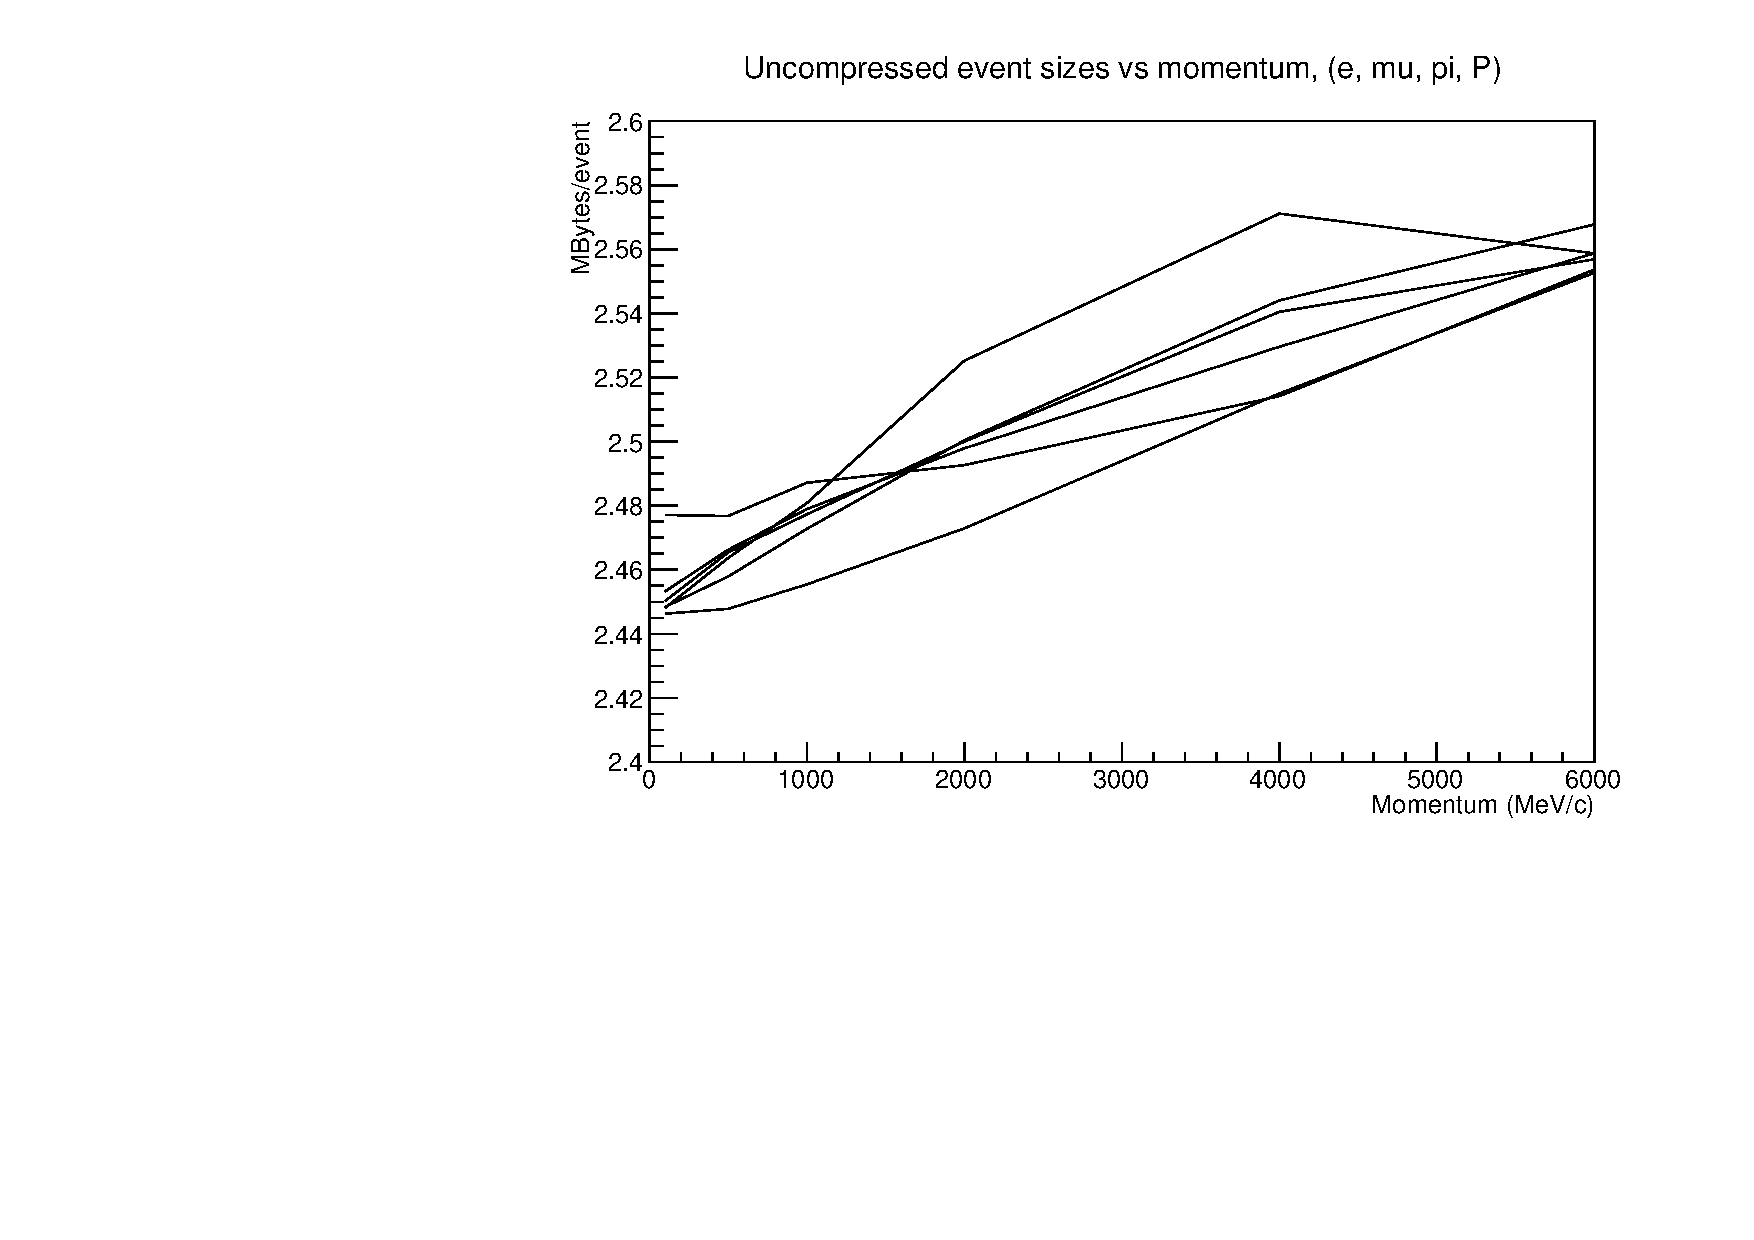
\includegraphics[width=0.3\textwidth]{btot.pdf}
  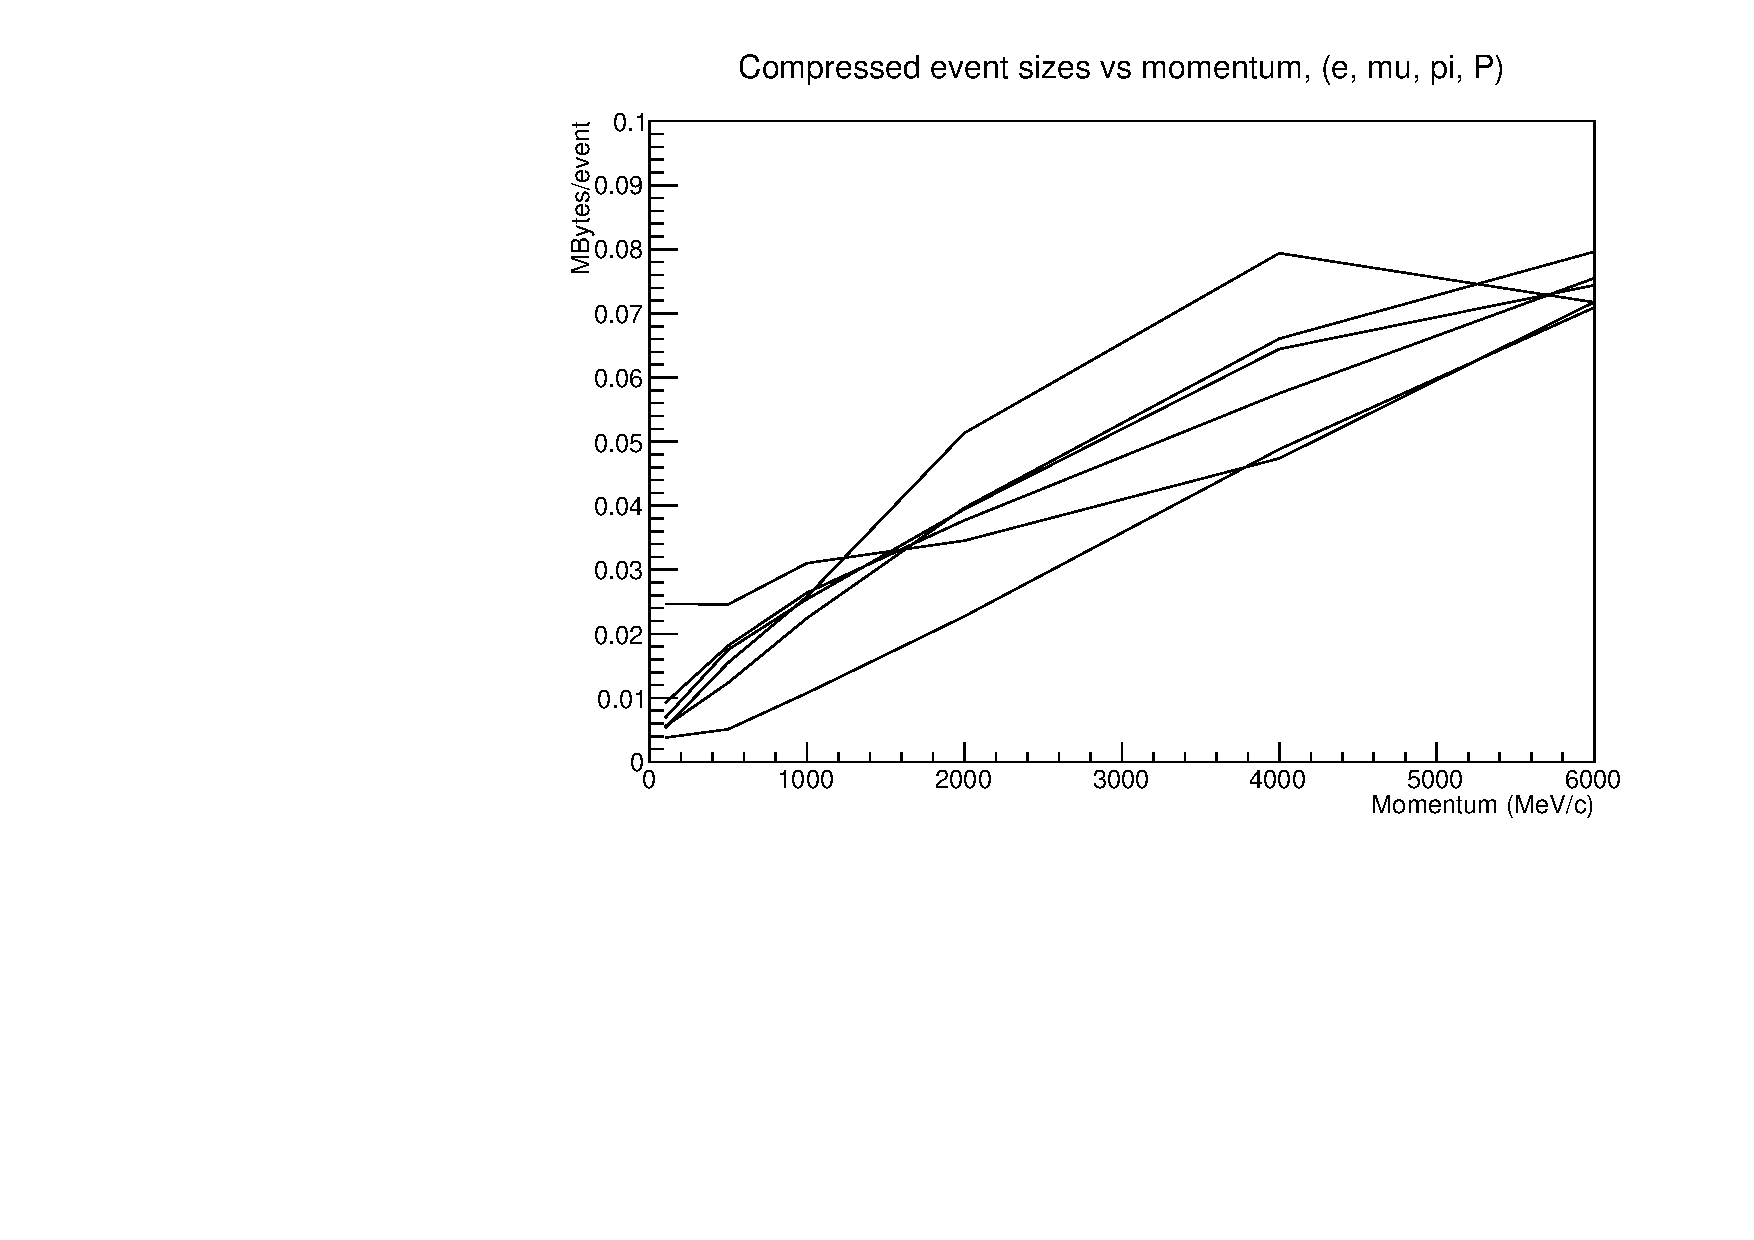
\includegraphics[width=0.3\textwidth]{bzip.pdf}
  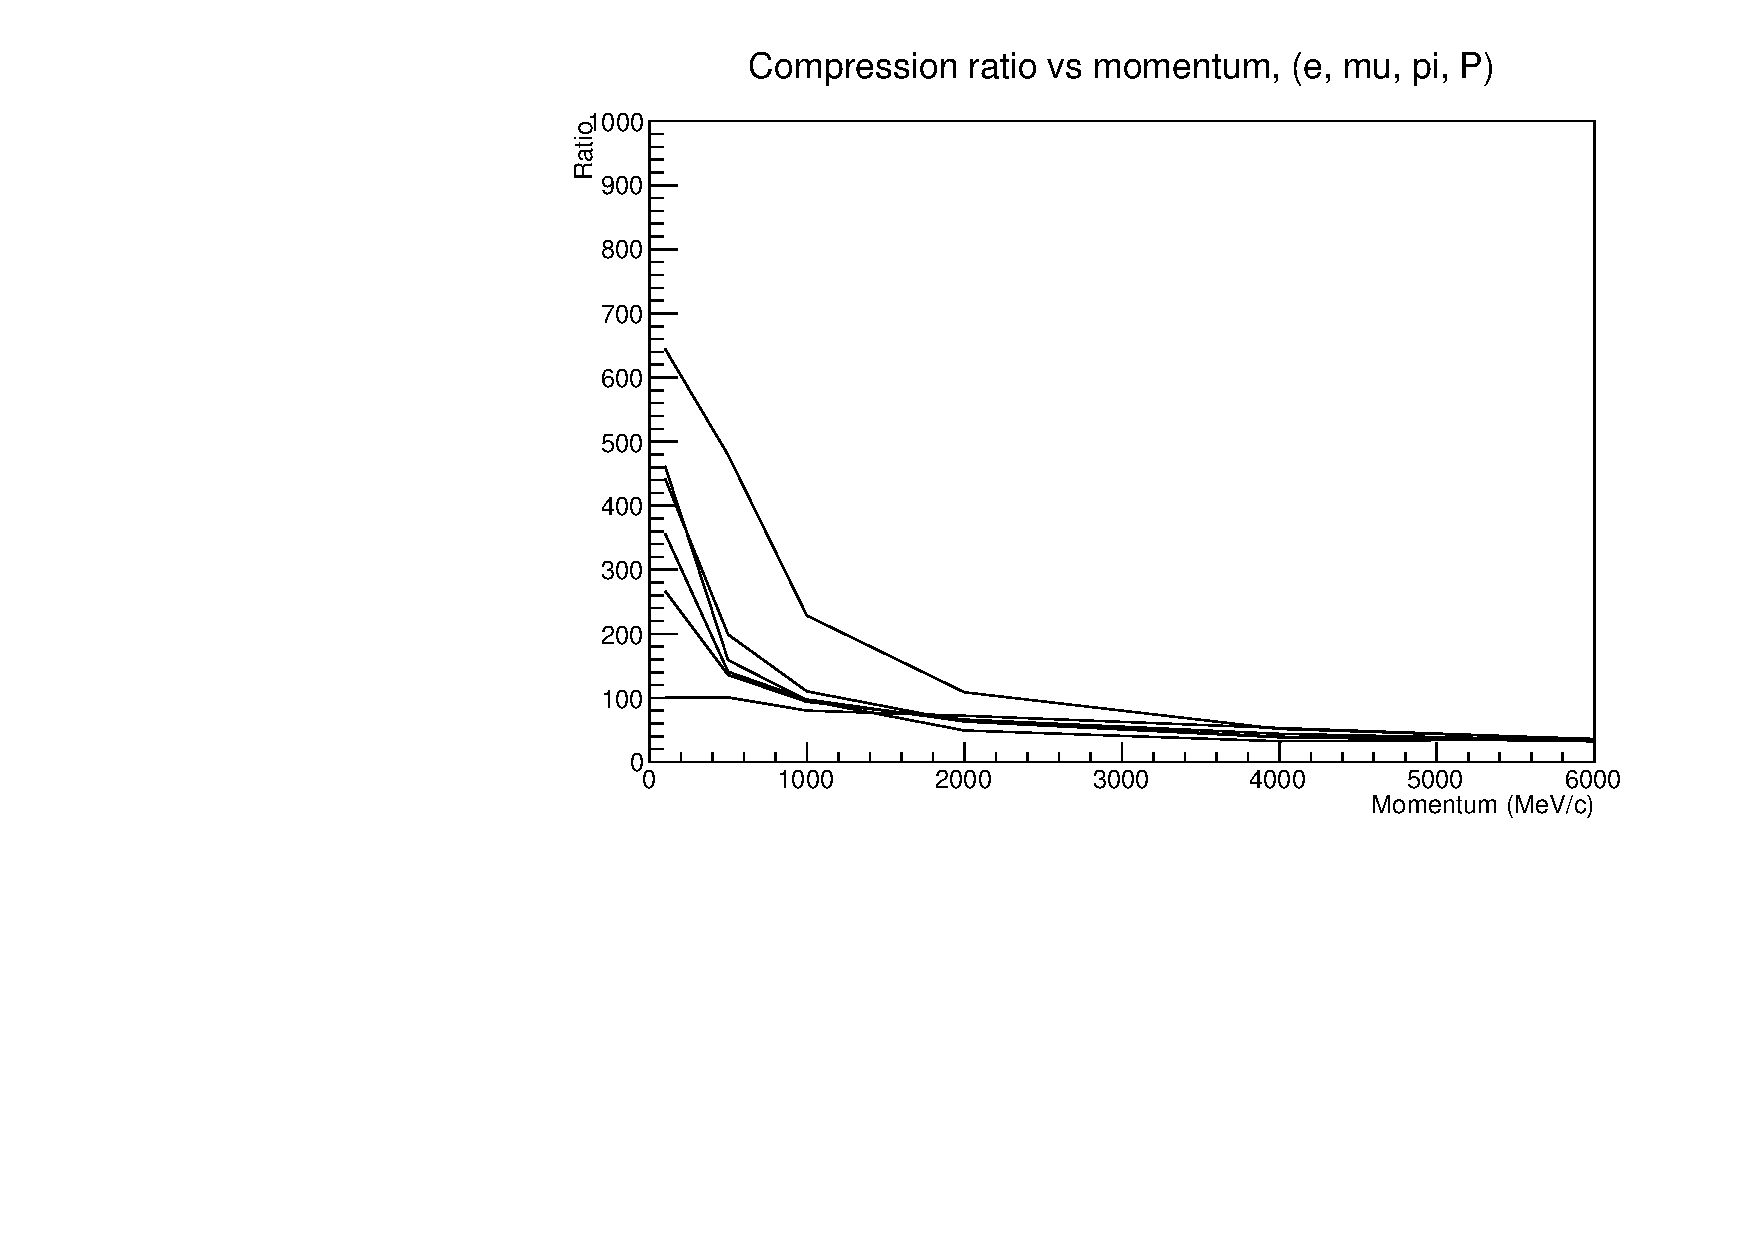
\includegraphics[width=0.3\textwidth]{brat.pdf}

\end{cdrfigure}

It must be noted that this exercise discovered the bulk of the
compressed data written by LArSoft is actually made up channel ID
numbers providing a data inflation of about a factor of 10.
For uncompressed data this added about 50\%.
There are also additional data elements related in the ``raw data''
branch which are superfluous or at best repeated more frequently than
is likely to be required.
In the LArSoft output, even though zero suppression is applied, every
channel has an associated a pedestal and a sigma as well as a
compression number.
There is also a sample count in addition to the one in the sample
vector which is stored.
These values do no vary yet each take up about the same (uncompressed)
size as the ADC values and are significant in size even after
compression.
They are not included in figure~\ref{fig:data-compression}.

Finally, as can be seen in the figure, the change in uncompressed
event size is only a minor function of event momenta and particle types.
It is believed that LArSoft is saving additional overhead for all
channels, even those that have been fully zero-suppressed.

The simulation used a detector consisting of \num{300000} wires and
thus naively the event size in the real detector would be some 5 times
larger.
However, given the arguments above, it is expected that this leads to
a gross over-estimate, possibly by one or two orders of magnitude from
what should be expected if even just a little effort is put into
designing a better storage schema.
Once compression is assumed, the problems with this sub-optimal
storage schema are lessened.
We then select the uncompressed event size to be \beameventsize and
the compressed event size of \beameventsizecompressed based
on~\ref{fig:data-compression}.
We identify this with being the zero-suppressed data produced by just
activity due to beam interactions or similar energy events and accept
the large over-estimation as a generous safety factor.






